\newpage
\section{Model Validation: Simulation Results}

The full nonlinear hybrid model is simulated with the initial conditions alone and the inputs ($u_1, u_2, F$ and $T$). The switching condition is not currently clear but assuming the goal of controller is to maximize the performance of the catalyst, the guard condition for switching to the saturated model is chosen to be the maximum $NO_x$ reduction among the saturated and desaturated models that is closed to the inlet $NO_x$. The hybrid automata for the system presented in the figure~\ref{fig::hybrid_automata}.

\begin{figure}[H]
        \centering
        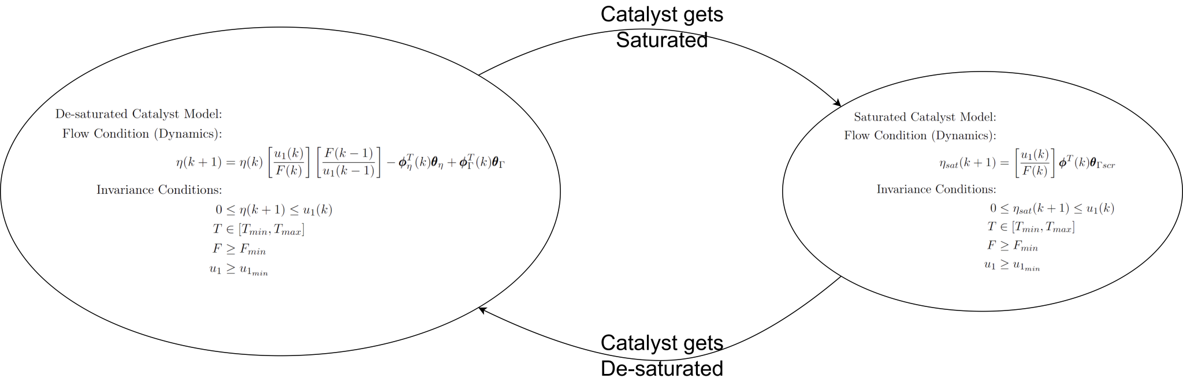
\includegraphics[width=0.75\textwidth]{\froot/figs/15_figs/hybrid_model.png}
        \caption{Hybrid automata describing the SCR-ASC system}
        \label{fig::hybrid_automata}
\end{figure}

We have the equations describing the hybrid model equation:
\begin{itemize}
\item De-saturated Catalyst Model:
\begin{align*}
        \text{Flow Condition (Dynamics):} &\\
                \eta(k+1) &= \eta(k) \lrb{\frac{u_1(k)}{F(k)}} \lrb{\frac{F(k-1)}{u_1(k-1)}}
                    - \pmb \phi^T_{\eta}(k) \pmb \theta_{\eta}  + \pmb \phi_{\Gamma}^T(k) \pmb \theta_{\Gamma}
                    \\
        \text{Invariance Conditions:} & \\
                0 &\leq \eta (k+1) \leq u_1(k)\\
                T &\in \lrb{T_{min}, T_{max}}\\
                F &\geq F_{min}\\
                u_1 &\geq u_{1_{min}}
\end{align*}
\item Saturated Catalyst Model:
\begin{align*}
        \text{Flow Condition (Dynamics):} & \\
                \eta_{sat}(k+1) &= \lrb{\frac{u_1(k)}{F(k)}} \pmb \phi^T(k) \pmb \theta_{\Gamma scr}\\
        \text{Invariance Conditions:} & \\
                0 &\leq \eta_{sat} (k+1) \leq u_1(k)\\
                T &\in \lrb{T_{min}, T_{max}}\\
                F &\geq F_{min}\\
                u_1 &\geq u_{1_{min}}
\end{align*}

\item The guard conditions for switching are still a work in progress. For the present work, the conditions is based on the objective of the closed-loop urea-dosing control system, i.e., maximizing $NO_x$ reduction at every time-step.
\begin{align*}
        \text{Saturated, if:} & \abs{u_1(k-1) - \eta_{sat}(k)} \leq \abs{u_1(k-1) - \eta(k)} \\
        \text{Desaturated, if:} & \abs{u_1(k-1) - \eta(k)} \leq \abs{u_1(k-1) - \eta_{sat}(k)}
\end{align*}
\end{itemize}


\subsection{Simulation Results}
The simulation results for the $NO_x$ reduction prediction per time step for all the tests are plotted below.

\begin{figure}[H]
        \begin{minipage}{0.49\textwidth}
                \begin{figure}[H]
                        \centering
                        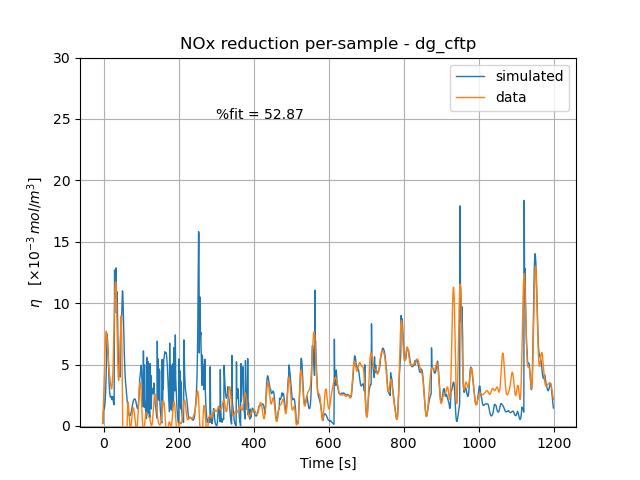
\includegraphics[width=\textwidth]{\froot/figs/15_figs/eta_sim_dg_cftp.png}
                \end{figure}
        \end{minipage}
        \begin{minipage}{0.49\textwidth}
                \begin{figure}[H]
                        \centering
                        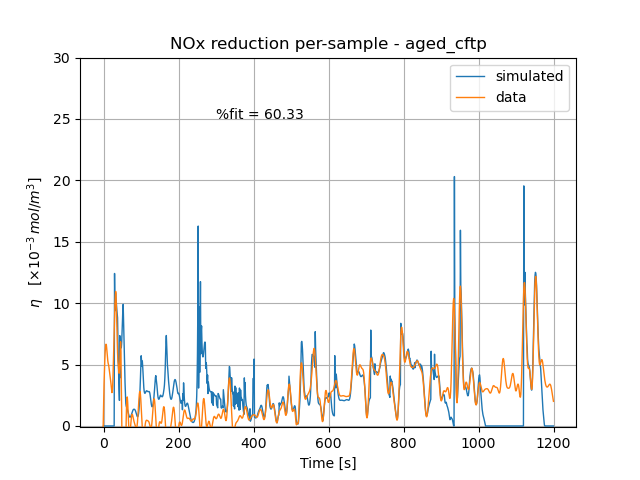
\includegraphics[width=\textwidth]{\froot/figs/15_figs/eta_sim_aged_cftp.png}
                \end{figure}
        \end{minipage}
        \caption{System response for cold FTP data}
\end{figure}

\begin{figure}[H]
        \begin{minipage}{0.49\textwidth}
                \begin{figure}[H]
                        \centering
                        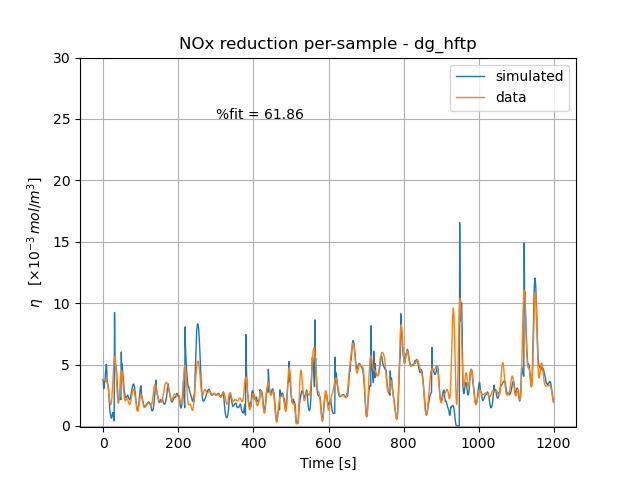
\includegraphics[width=\textwidth]{\froot/figs/15_figs/eta_sim_dg_hftp.png}
                \end{figure}
        \end{minipage}
        \begin{minipage}{0.49\textwidth}
                \begin{figure}[H]
                        \centering
                        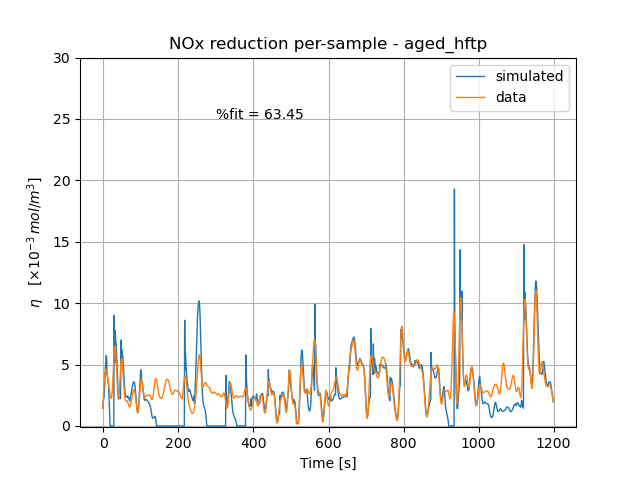
\includegraphics[width=\textwidth]{\froot/figs/15_figs/eta_sim_aged_hftp.png}
                \end{figure}
        \end{minipage}
        \caption{System response for hot FTP data}
\end{figure}

\begin{figure}[H]
        \begin{minipage}{0.49\textwidth}
                \begin{figure}[H]
                        \centering
                        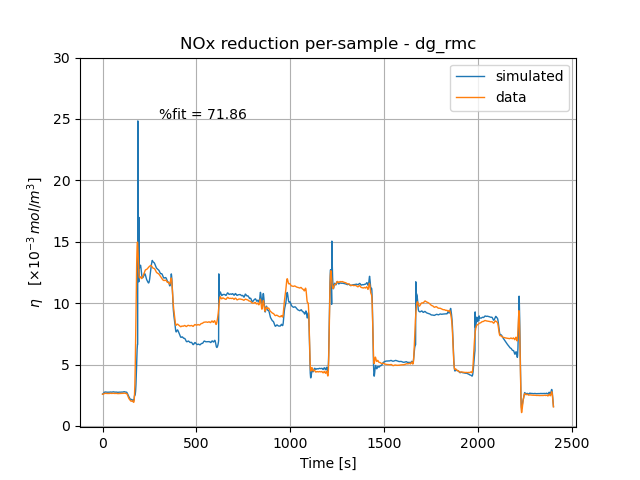
\includegraphics[width=\textwidth]{\froot/figs/15_figs/eta_sim_dg_rmc.png}
                \end{figure}
        \end{minipage}
        \begin{minipage}{0.49\textwidth}
                \begin{figure}[H]
                        \centering
                        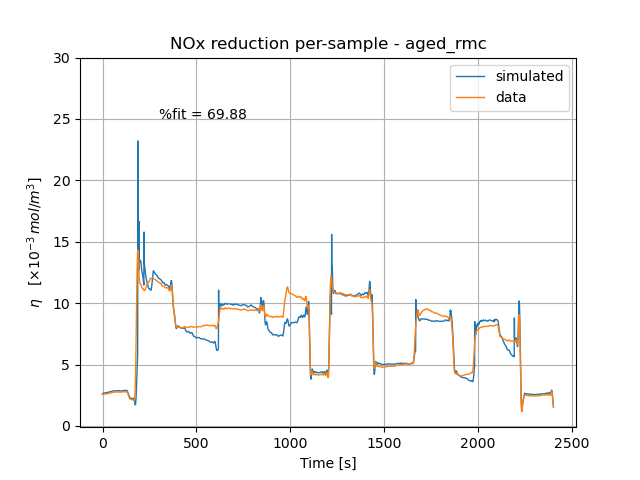
\includegraphics[width=\textwidth]{\froot/figs/15_figs/eta_sim_aged_rmc.png}
                \end{figure}
        \end{minipage}
        \caption{System response for RMC data}
\end{figure}


\begin{table}[H]
        \centering
        \caption{$\%$fit of the models with test data}
        \label{tab::results}
        \begin{tabular}{l l c c}
                \hline \hline
                Age & Test & Switched Nonlinear Model & Linearized CSTR Model \\ \hline \hline
                Degreened & RMC & 71.86 & 19.98 \\
                Aged      & RMC & 69.88 & 27.66 \\ \hline
                % =========================================
                Degreened & hot FTP & 61.86 & 7.10 \\
                Aged      & hot FTP & 63.45 & 7.38 \\ \hline
                % =========================================
                Degreened & Cold FTP & 52.87 & 23.24 \\
                Aged      & Cold FTP & 60.33 & 23.19 \\ \hline
                \hline
        \end{tabular}

        $\%fit = 100 \times \lr{1 - \frac{\norm{Y- \hat Y}}{\norm{Y -
        mean(Y)}}}$ \\
        $\%fit$ is the percentage of the measured output that was explained by the
        model.
\end{table}

Thus, the switched nonlinear model consistently fits the data with a goodness of fit value greater than $50\%$ for all
the test-cases. While the linearized CSTR model, though identifiable, has no further room for improvement in terms of
model refinement, the proposed hybrid nonlinear model has further potential for refinement resulting in lower prediction
errors than presented. Specifically, further work needs to be done in the development of appropriate switching
conditions between the saturated and desaturated models. Moreover, the model offers the flexibility of incorporating
more complex models of underlying physical properties (rate-constants, residence time, etc.) relaxing or reworking the
assumptions to better fit the operating conditions.

